\newif\ifshowsolutions
\showsolutionstrue
\documentclass{article}
\usepackage{listings}
\usepackage{amsmath}
%\usepackage{subfigure}
\usepackage{subfig}
\usepackage{amsthm}
\usepackage{amsmath}
\usepackage{amssymb}
\usepackage{graphicx}
\usepackage{mdwlist}
\usepackage[colorlinks=true]{hyperref}
\usepackage{geometry}
\usepackage{titlesec}
\geometry{margin=1in}
\geometry{headheight=2in}
\geometry{top=2in}
\usepackage{palatino}
\usepackage{mathrsfs}
\usepackage{fancyhdr}
\usepackage{paralist}
\usepackage{todonotes}
\setlength{\marginparwidth}{2.15cm}
\usepackage{tikz}
\usetikzlibrary{positioning,shapes,backgrounds}
\usepackage{float} % Place figures where you ACTUALLY want it
\usepackage{comment} % a hack to toggle sections
\usepackage{ifthen}
\usepackage{mdframed}
\usepackage{verbatim}
\usepackage[strings]{underscore}
\usepackage{listings}
\usepackage{bbm}
\rhead{}
\lhead{}

\renewcommand{\baselinestretch}{1.15}

% Shortcuts for commonly used operators
\newcommand{\E}{\mathbb{E}}
\newcommand{\Var}{\operatorname{Var}}
\newcommand{\Cov}{\operatorname{Cov}}
\newcommand{\Bias}{\operatorname{Bias}}
\DeclareMathOperator{\argmin}{arg\,min}
\DeclareMathOperator{\argmax}{arg\,max}

% do not number subsection and below
\setcounter{secnumdepth}{1}

% custom format subsection
\titleformat*{\subsection}{\large\bfseries}

% set up the \question shortcut
\newcounter{question}[section]
\newenvironment{question}[1][]
  {\refstepcounter{question}\par\addvspace{1em}\textbf{Question~\Alph{question}\!
    \ifthenelse{\equal{#1}{}}{}{ [#1 points]}: }}
    {\par\vspace{\baselineskip}}

\newcounter{subquestion}[question]
\newenvironment{subquestion}[1][]
  {\refstepcounter{subquestion}\par\medskip\textbf{\roman{subquestion}.\!
    \ifthenelse{\equal{#1}{}}{}{ [#1 points]:}} }
  {\par\addvspace{\baselineskip}}

\titlespacing\section{0pt}{12pt plus 2pt minus 2pt}{0pt plus 2pt minus 2pt}
\titlespacing\subsection{0pt}{12pt plus 4pt minus 2pt}{0pt plus 2pt minus 2pt}
\titlespacing\subsubsection{0pt}{12pt plus 4pt minus 2pt}{0pt plus 2pt minus 2pt}


\newenvironment{hint}[1][]
  {\begin{em}\textbf{Hint: }}{\end{em}}

\ifshowsolutions
  \newenvironment{solution}[1][]
    {\par\medskip \begin{mdframed}\textbf{Solution~\Alph{question}#1:} \begin{em}}
    {\end{em}\medskip\end{mdframed}\medskip}
  \newenvironment{subsolution}[1][]
    {\par\medskip \begin{mdframed}\textbf{Solution~\Alph{question}#1.\roman{subquestion}:} \begin{em}}
    {\end{em}\medskip\end{mdframed}\medskip}
\else
  \excludecomment{solution}
  \excludecomment{subsolution}
\fi

\newcommand{\boldline}[1]{\underline{\textbf{#1}}}

\chead{%
  {\vbox{%
      \vspace{2mm}
      \large
      Kelsi Riley \& Sakthi Vetrivel \hfill
      Caltech Earthquakes \hfill \\[1pt]
      Machine Learning \& Data Mining \hfill
      Caltech CS/CNS/EE 155 \hfill \\[1pt]
      Miniproject 3\hfill
      March $12^{th}$, 2018 \\
    }
  }
}

\begin{document}
\pagestyle{fancy}

% LaTeX is simple if you have a good template to work with! To use this document, simply fill in your text where we have indicated. To write mathematical notation in a fancy style, just write the notation inside enclosing $dollar signs$.

% For example:
% $y = x^2 + 2x + 1$

% For help with LaTeX, please feel free to see a TA!



\section{Introduction}
\medskip
\begin{itemize}

    \item \boldline{Group members} \\
    Kelsi Riley \\
    Sakthi Vetrivel
    
    \item \boldline{Team name} \\
    Caltech Earthquakes
    
    \item \boldline{Division of labour} \\
    % Insert text here.
    Kelsi implemented the HMM, and focused on improving it. She also did the preprocessing for the HMM, and was responsible for the unsupervised training of the HMM. Sakthi implemented the RNN and worked on improvements for it, as well and the visualization and interpretation of the HMM.
    \item \boldline{Github Repository} https://github.com/kelsi-riley/project3/

\end{itemize}



\section{Pre-Processing}
\medskip
For our pre-processing of Shakespeare's sonnets, we started by converting each poem into a list, where the list contains the words of the poem in order of appearance, with a newline character between lines of the poem. Then because our HMM uses integer representations of emissions, we created two dictionaries: one mapping words to unique integer values and another mapping integers to unique words. This initial preprocessing was helpful, but when we looked at the values stored in our dictionaries, we realized that capitalized and lowercase words were considered different emissions with this processing, and if a word was followed by punctuation, it was considered a different emission than if it was not.

This prompted us to make each word lower case as we processed it, to ensure that words are considered the same emission regardless of their capitalization. We also decided to remove the characters '.', ',', ':', ';', '(', ')' and '?' from the poems we processed so that we didn't have many different emissions associated with the same word. We decided to leave in the apostrophe due to its presence in contractions, and actually being a part of the representation of the word. This updated preprocessing was an improvement from our initial attempt, but ultimately fell short of what we needed due to the presence of phrases in quotations in some of the poems (i.e. 'Will' in sonnets 135 and 136 and 'not you' and 'I hate' in sonnet 145). This lead us to need to adopt a somewhat more complicated process for removing quotations around words.

We ultimately ended up deciding to remove an apostrophe if it was in the beginning of a word and the word was not a word we recognized as beginning with an apostrophe. Then, we would remove the next apostrophe in the line. This allowed us to remove the quotations around certain words and phrases in the poems and simplified the number of observations of our model. 

Because sonnets 126 and 99 adhered to the structure of a sonnet much less rigidly then the rest of Shakespeare's works, we decided not to train our models on them. While we were pre-processing the poems, we then did not represent these poems in our produced list of poems, where each poem was represented as a list of integers. 

Also, as we suspected it would be useful to be able to easily assess if an integer emission mapped to the newline character, we decided to initialize our dictionaries mapping words to their unique integer representations and vice-versa with the newline-0 pair. This would allow us to easily identify when we had reached the end of the line when generating poems, instead of having to constantly use the dictionary mapping integer representations to strings to check if the string mapped to is the newline character. 

Finally, we wanted to be able to generate sonnets that rhyme, so we ended up extending our pre-processing to enable doing so. To do this, we used our knowledge of the rhyme scheme of Shakespearian sonnets: abab cdcd efef gg. Then, as we processed our poems, we added the unique integer representations of last words of lines that rhyme to a rhyming dictionary. This rhyming dictionary mapped unique integer representations of words to a list of the integer representations of words that it rhymes with. We considered altering this so that if two words rhyme with each other, then every word that rhymes with either of them will rhyme with both of them, but ultimately decided against this implementation due to Shakespeare's liberal use of slant rhymes. We thought that generalizing rhyming this way could possibly produce "rhymes" that hardly resemble rhymes at all. 




% Explain your data pre-processing choices, as well as why you chose these choices initially. What was your final pre-processing? How did you tokenize your words, and split up the data into separate sequences? What changed as you continued on your project? What did you try that didn't work? Also write about any analysis you did on the dataset to help you make these decisions.

\section{Unsupervised Learning}
\medskip
For our implementation of unsupervised learning for our Hidden Markov Model, we used the Homework 6 Solution Set. This implementation used the Baum-Welch algorithm to train on an unlabeled data set. We experimented with a variety of hidden state and iteration counts, and ultimately ended up deciding to choose these values to balance quality of poem emission with computation time. A greater number of hidden states seemed to yield more convincing imitation sonnets, but also produced very long run times. We ended up deciding to settle for 16 hidden states and modified our code so that trained Hidden Markov Models could be stored in text files and then accessed again later, so that we wouldn't have to wait for hours every time we wanted to generate poems. 

\subsection{Choosing Hidden States}
\noindent
\textbf{Poem generated from HMM with 8 Hidden States:}\\
Seen is when now pretty importune air \\
Even the dial in the and eye do \\
To in sadly amen telling lend fair \\
Needing them as the one of leisure too \\
Others himself whose much weary three cold \\
Own alteration urge torn is to thee \\
Best urge when heavily of my make old \\
Because loves see in end pyramids me \\
And my are mind of glass good your which jewel \\ 
Worth say few frequent thy in thy eyes those \\
Yet unlooked then to rehearse which that cruel \\
It away essays is with more strong grows \\
\indent
  Say to whom strongly drawn full things what fitted \\ 
\indent
  Blame sick of a prove of else crime committed \\

\clearpage

\noindent
\textbf{Poem Generated from HMM with 12 Hidden States:} \\
Essays slay comment tear though all not show \\
Hours would neglected to beauty thou hearts \\
Boot to of the lives mad to in dost so \\
I thoughts interest of no thoughts is the line\\ 
Of that two authorizing no one her \\
Self-love simple being therein not truth this \\
End a thou that thy say when thy am her \\
Which said when your sweet shall love to see is \\
Beauty thinking since with to gain hours \\
I use did know with taste let wrongs thou one \\
My jade of soon so jewels be flowers \\
Alone confound without said thy alone \\
\indent
  Then flattery doth being an love deeds be\\ 
\indent
  You largess bid sums my self bad when I \\
 
\noindent 
\textbf{Poem Generated from HMM with 16 Hidden States:}\\
Far phrase unhappily whom high thou heart \\
Are and carve bareness fragrant not all make \\ 
Two lawful not remembrance herald art \\
By and wrinkles the welfare break sense take \\
Knows for tells false heart where eye hue and know \\
Ills and wink heart his being is catch be \\
Proved I of my assured moiety so \\
Live have was constancy doth think in I \\ 
I stay a for too you thy not self man \\
Heaven's age out thou I doth tell pilgrimage \\
Watch o in the time's fair with loving can \\
War for all a pent that when my you age \\
\indent
  Is saw is soul richly cannot days heart \\
\indent
  Or since the thy cloak we thou call wide art \\

As we increased the number of hidden states of our Hidden Markov Model, the quality of poem generated seemed to improve. Note: these poems were generated using our more sophisticated emission generation method, which enforces that lines must all be 10 syllables and that the produced poem must follow the proper rhyme scheme. We qualitatively decided that training with more hidden states improved the performance of our model, and ended up only using 16 hidden states instead of exploring the potential of using more because training the Hidden Markov Model with 16 hidden states already took hours. We thought training a Hidden Markov Model with any more hidden states would take too long to be practical. 
% This section should highlight your HMM. What packages did you use, if any? How did you choose the number of hidden states?



\section{Poetry Generation, Part 1: Hidden Markov Models}
\medskip
% Describe your algorithm for generating the 14-line sonnet. As an example, include at least one sonnet generated from your unsupervised trained HMM. You should comment on the quality of geneating poems in this naive manner. How accurate is the rhyme, rythym, and syllable count, compared to what a sonnet should be? Do your poems make any sense? Do they retain Shakespeare's original voice? How does training with different numbers of hidden states affect the poems generated (in a qualitative manner)? For the good qualities that you describe, also discuss how you think the HMM was able to capture these qualities.
For our naive 14-line sonnet generation, we simply generated poems by randomly selecting a hidden state to start with, then randomly selecting the next observation and next state using the previous hidden state, as well as transition and emission probabilities stored in A and O of the Hidden Markov Model. We continued to do this until we had added 14 newline characters to our emission, so it would be 14 lines long. Poems generated this way were pretty terrible attempts at imitating sonnets. I have included a few examples of sonnets produced this way:

\subsection{Poems Naively Generated from HMM with 8 Hidden States, Trained for 400 Iterations} 
\noindent
\textbf{Sonnet 1} \\
Shines to \\
Wrong vanished when at and reason more had being and departest canst time in his tempteth \\
Painted goddess I \\
Said hours sight lesser the all to blessed suppose brief thy with lays lo in thine took I absent to \\
Age bosom aye or none \\
Name to of days with woe the keep even wit on from though \\
Making it sealed against \\
Grief to to those \\
\\
Afterwards her but and \\
Hast I all \\
Ornament my \\
\indent
  Glass the her confined all longer not have as \\
\indent
  Sing it knife spite by love is \\
  
\noindent
\textbf{Sonnet 2} \\
And the spurring and that and \\
Spirit in press I those brow a is the to you how and \\
\\
\\
Lies can doth sorrow to eager pluck bending \\
Iniquity course love she fiend sweet gain poor moon thy \\
Deeds born believe all as years fresh to the eternal interest but so glad be hath the sunset swear \\
Black put and that \\
Still have state my may do that such have no thou a sweet himself how salving \\
Is it hence secret purity thy unkind past read \\
Fresh shall as no or decease sun refined costly truth inward with \\
Sweet this what \\
\indent
  Saw so love lose wish wait who \\
\indent
  Thing my by shadow the I \\

As you can see, the syllable count of the lines is very inconsistent, ranging from 0 (in the case of the completely empty line) to nearly double the expected syllable count. On a similar note, the rhythm is inconsistent with the Shakespearian sonnets we used to train our HMM. This naive generation also fails to include any rhyming at all. Overall, these generations were largely nonsensical and fail to be very understandable. As such, they fail to retain Shakespeare's original voice very well and don't resemble his Sonnets closely at all. When we use this same generation method with a Hidden Markov Model with more hidden states we see similar results:

\subsection{Poems Naively Generated from HMM with 16 Hidden States, Trained for 400 Iterations}
\noindent
\textbf{Sonnet 3} \\
Self of ere \\
Write silence sun worth things my in absence or \\
\\
Sour account which love\\ 
Sake my blind therein he by by hand world's thy full \\ 
Rotten I not flowers then I I and err who I as \\
Rents wake and ere decease done lines every of simple and \\
Will to eyes moon incertainty king invent doth print a what like \\
Stands forgotten ever have thee poor \\
Verse false or \\
Possessing love's the and \\ 
Desired if \\
\indent
  See this in all my \\
  \\
  
\noindent
\textbf{Sonnet 4} \\
Beams it but grace thee for but shore their make with thoughts than \\
Kept body hadst thou profitless \\
Be should pricked all to that \\
Thee the simply \\
Hid bath in despite worth his a true and learn be even when \\
Eclipses thee to sweetly themselves are \\
Show this of which farther moon \\
Acquainted all praise to \\
You their live \\
Loving tender your will as heart unkindness yet \\
Too true it deceive once friends all it she lose earth upon now he happy be \\
Is not may mistress' all from hath \\
\indent
  More so \\
\indent
  Jewel and\\

When we increase the number of hidden states, the length of the lines becomes more consistent, and there are fewer lines that don't contain any words at all, but the produced sonnets are still fail to meaningfully resemble Shakespearian sonnets. The quality improves with the increase in hidden states, but ultimately the problems of the generated sonnets failing to rhyme, have the correct number of syllables, and adhere to the standard rhythm of sonnets makes these generations lackluster. With more hidden states, Shakespeare's voice appears to show in the generation better, but it still isn't very accurately represented by our generations. 


\section{Poetry Generation, Part 2: Recurrent Neural Networks}
\medskip

% Explain in detail what model you implemented and using what packages. What parameters did you tune? Comment on the poems that your model produced. Does the LSTM successfully learn sentence structure and/or sonnet structure? How does an LSTM compare in poem quality to the HMM? How does it compare in runtime/amount of training data needed to the HMM? Include generated poems using temperatures of 1.5, 0.75, and 0.25 with the following initial 40-character seed: ``shall i compare thee to a summer\'��s day\n'', and comment on their differences.

\subsection{Initial Implementation}
For our preprocessing for the RNN, we decided to first break down the text file by line, and for each line we parsed, we made sure the line was not empty (not just an endline character) and removed any special characters from it. For example, we wanted to "Hello!" and "hello" to be processed as the same sequence of characters. We then finished each line with an endline character and added it to a accumulating string, which held the contents of the processed text file. After processing the input, we created dictionaries to convert each character found in the processed text to an integer, and a dictionary that converted integers to characters. We then generated a data set splitting this string into sequences of 40 consecutive characters, and converting the sequence of characters into a sequence of integers, and used the 41st character of the sequence as the y value, again, after converting it to an int.

We implemented a recurrent neural network using the Keras package for Python3. Using a sequential model, we had two dense LSTM layers of size 200, and one output layer. We calculated our loss using categorical cross-entropy loss, and 'adam' optimization. We also fine tuned our batch size, testing values of 32, 64, and 128. By observing the poems produced for these batch sized after 10 epochs of training, we settled on a batch size of 64. We also fine-tuned the size of the LSTM layers, trying sizes of 100, 150, and 200, as suggest in the project details, and settled of a size of 200. We then trained this model for 125 epochs, converging to a loss of 0.4146 from a loss of 3.45 after the first epoch. To improve our model, we also looked at more complex RNN, using two dropout layers between the LSTM layers, and fine tuned the dropout probability to eventually choose 0.4. Initially, the model was only trained for 20 epochs, but we found that the loss still hadn't converged so we continued training until the loss did not improve for 2 epochs. We used a window size of 40 as the instruction suggested, but later moved to smaller window size of 25 in our attempts to improve our model. 

To generate our poems, we used our seed sequence "Shall I compare thee to a summer's day?" and processed it, and for a sliding window of 40 characters, predicted the next letter in the sequence. Our model gives us an array of probabilities for the next character, given the previous 40 characters, so using this array of probabilities, we sample from the population of characters accordingly for a given diversity value. We also counted the number of newline characters that were predicted in the entire generation process, stopping after 14 newline characters, giving us 14 lines in the poem. 

Despite training for so many iterations, our LSTM did not successfully learn sentence structure or sonnet structure, as we see in the poems below, few of the words produced are real words. However, for the brief segments of the poems that contain real words, it seems to follow some loose sentence structure. For example: "i love you" and "of the braid". As a result, the poem quality seems fairly low, and this is a direct result of the character-based nature of the neural network resulting in jumbled English. Because there are so many more sequences of characters than sequences of words, the RNN takes more training data to train, but both sets of training data were still generated from the same text file. It took much longer to train the RNN than to train the HMM, again, because it starts from a lower level of understanding, since we are working with characters instead of words. 

\subsection{Poems}

\noindent
----- diversity: 1.5\\
----- Generating with seed: "  shall i compare thee to a summers day\\
"\\
  shall i compare thee to a summers day\\
weat kerp tellv in these i would to hath\\
my self iil iiddsu your thlltt my self brane ereed\\
but ceatt that weal i love you be teildde\\
and me altereasonse of the braid and lind\\
which treals mind eye is is a lawvereo\\
at tenmn lines bety paming iimeshsy\\
or at dolg pdr tiat weadddleditg tiink\\
eor shamls iampeut sp will he's shcd might\\
sevoy seep tidu thou 'liserpeas nor\\
j thak oyck tine suelt so lem so ku haln\\
  and nock i tas of fold cach or pattry\\
but be thy liate me thrnugh mights me sn botn\\
and in holaskeri hrln with the trwe doth green\\
and confoundane farth in thee tie live"\\


\noindent
----- diversity: 0.75\\
----- Generating with seed: "  shall i compare thee to a summers day\\
"\\
  shall i compare thee to a summers day\\
when that wilt nottncry that fell asd feidt\\
  that it 'bol gor moctatd i do dispilts\\
  and diary my self i'ck tren to the most\\
  but when your changent of this weil\\
byt sickt his tputatt mot i loow more eeee\\
to say toe borcmest whereup the bear\\
thy presclv ceauies ifart he lile artire\\
for whose winter's enoling on the rulp're\\
when sesimg a betteiry ocrure of thy deeds\\
therefo thy putlok dead trealed thou art\\
o what a worthsed wron delive no mane sehmnts\\
oo aly of these falsehe move's fresh ceserity\\
then the means me with vinter did stansed\\
and dotnt and in habkt and it gaults light"\\


\noindent
----- diversity: 0.25\\
----- Generating with seed: "  shall i compare thee to a summers day\\
"\\
  shall i compare thee to a summers day\\
aid uosthfr this wirte doth beauty stail\\
  thou mayst be thy oudsent'st a linit sade\\
  but when your count in these cannot chind\\
o carve norer mine him though mews the even\\
  but day doth daily draw my sorrows line\\
so thy freat gift woon be forgouingnl\\
for higheo of line ow well my heart deegines\\
so fotth the blow of with dupy steet selbit\\
  ald my hoade fyen siln liss lysbs'bd and were orisit\\
oatt reason haved the stard or thy sweet graces\\
beauteous all fellls tine world have erreemed\\
more that my self but was donf iis oun\\
gow many lambs kild and they acvodance seegng\\
and all the dead no nore drtbl dole"\\

\section{Additional Goals With RNN Model}
\medskip

% Explore methods of improving your poems or extending them. You do not need to attempt all of the tasks listed in the assignment for full marks on this section. If you have ideas for other improvements to the poetry generation not listed here, feel free to talk to a TA and work on it. The sky is the limit.

\subsection{Haikus}

We adapted our RNN to compose haikus. To do this, we created an file of haikus, where each line in a haiku in separated by a tab character, and each haiku is separated by a newline character. We also changed our window size from 40 characters to 15, since haikus are much smaller, and a 40 character seed would make up a significant portion of the poem. We continued to use LSTM layers of size 200. We then trained the RNN on this data set for about 100 epochs with a batch size of 64 (the batch size we found was effective for our sonnets). To generate our haikus, we used the same skeleton as the sonnets, just adjusting the window size. The results for the haikus were much more promising than the sonnets, which was surprising considering the training set was smaller. Here are some of our favorite haikus that were generated:\\

\begin{center}

light snowy breath	to read\\
old tombstones hot wind shadows\\
the roadrunner's beak\\

\bigskip

\noindent
furled umbrella\\
turns into a cane\\
chernobyl vells\\

\end{center}
 
Of course, many of the haikus we generated often contained just jumbled letters, and when they did contain words, they rarely made sense, much like the haikus above. However, the model was able to predict syllable count fairly accurately, as you can see the first haiku follows the 5-7-5 pattern, and the second haiku is close. Given more time, we would have liked to experiment with the Word2Vec package and worked to predict words that were similar to the previous words in the sequence.


\subsection{More Complex RNNs}

To improve our RNN, we decided to implement a more complex model. Instead of just using two LSTM layers of size 200, we decided to include dropout layers as well to avoid overfitting.We also used a smaller window size of 25. Thus our final RNN model consisted of two alternating LSTM layers of size 512, alternating with dropout layers. For these dropout layers, we experimented with probabilities of 0.1, 0.2,, 0.4, and 0.5, settling on 0.2. Moreover, instead of predicting the character following a sequence, we trained the model to predict the character preceding the sequence. This was in preparation for us to generate rhyming poems.

Given the chance to do this again, we would have liked to also train with a validation set, and have stopped training when the validation loss stopped improving, instead of depending of the training loss. Here are the poems generated with this approach:

\medskip


\begin{flushleft}
----- Generating with end: ue by the grave and thee\\
----- Diversity: 0.25\\

\medskip
and in this cold complaining\\
she would have trained crie\\
and in his and he like again\\
my art thou art in me must roves to side thy state\\
and in your offences fived in your devory\\
of fathered bester and with dinkilling eye\\
that she more living so offence alove\\
in either kill of beauty tend\\
and with a concestion makes her wind\\
and with your shame to supretise is scapening on to love my love\\
that my after for my days dad make the mettle wit\\
against my valthough it should nor gistless\\
cinfounded in a mined eyes\\
the tongue by the grave and thee\\
\medskip
\clearpage


----- Diversity: 0.75\\
\medskip
but loves her painted hend\\
with whose what eyes now love to my\\
and that can men shall heavenly for see only most to shows and toney\\
to make the mudder's grace\\
for thy sweet to time's eyes to hast\\
but no so is my love to cay\\
and to the humbers at the spirit on thee\\
'didst thou the sefle but in his rain\\
to from the best this true for then the eye alone\\
even in my love com from that at the reason\\
to lives my sorrow nature had't teou poy\\
to fair thy loses she lacks and unneed the bound to make their sidness\\
fit and the trembling eyes\\
the tongue by the grave and thee\\
\medskip
----- Diversity: 1.5\\
\medskip
i should in cartle's dame\\
was fined in lidob giden kies\\
then boldness her beauteous i will\\
hinour to elmantinal condensmaking\\
with those and burd nor let\\
to prubify to leave th from it\\
when shalt thou my have be end\\
so do am state at living eye and heart it may be gone
lix\\
the other hours are so co civitate\\
the colous o'erds to hell for love and bift from this all treed\\
and when that gave to trespect thy state\\
but were the had taught the cloud or all apay\\
and in her hourffece baskys-are tongue by the grave and thee\\
\end{flushleft}

\subsection{Larger Training Set}

In order to give the RNN more information to train on, we decided to include another file along with the spencer file given to us. Finding other sonnets composed by Shakespeare, we decided to process that text as well and include it to train our model. This larger training set was used in our final RNN model.


\subsection{Rhyming}

For our rhyming using the RNN, we used this implementation of the more complex RNN. Our first step was to generate a rhyming dictionary using the CMU dictionary and parsing each line of the sonnets. Using the CMU dictionary, we generated the pronunciations of each of the words in the Shakespearean texts, and compared the pronunciations of the ending of each of the words, so each word mapped to the pronunciation of its ending, and each pronunciation mapped to a list of words with that ending. 

Now to generate the rhyming poem, we find the endings of each line and generate the preceding characters based on the word. First, we find 7 random words in the sonnets, and make these the ends of lines 1, 2, 5, 6, 9, 10, and 13. Then, we use our rhyming dictionary to choose a word that rhymes with the line endings of the aforementioned lines and make these words the endings of lines 3, 4, 7, 8, 11, 12, and 14, such that we have a $ababcdcdefefgg$ rhyme scheme. 

Below is one of the poems generated through this process:\\
\\
Have women witagainst the cause but in the horn,\\
The sparm'dall wither yet love me all contented stair,\\
To beand croused could back their mildress' sky forlorn,\\
Effects and dischance andmore beauty of thyself all stair.\\
But his smokest love some is and now appear,\\
With that praise for living chance or thy burn,\\
Friendand for thee and steared berience more you peer,\\
Lively and confounds his artand heavenly one can spurn.\\
That true whan attening of her lind and horse,\\
Thas thoosebut if the would be maunt the heart,\\
Of all love's sout'st she dings with thy scarce,\\
Eyesand never was so watch the for both's transport.\\
\indent
To the priseand sily burupt make tears they sphere,\\
\indent
Thoutment on that gave darefrown from the dangerous year.\\


\section{Additional Goals with HMM Model}
\subsection{Syllable Count}
To generate emissions that more closely resembled sonnets, we decided the first thing that we needed to do would be to make sure generated lines have the proper number of syllables. To do this, we created a new poem generation function that produced lines that were all 10 syllables. To do this, we simply generated the beginning of lines as usual, but kept track of the syllable count of our line. We would not add the newline character until our line contained exactly 10 syllables, and would not add a word to our line if it would cause us to surpass 10 syllables. This implementation would also "backtrack" or remove words we already added to the line if it could not find a word to add to the end of the line after many attempts. 

This new generation method ultimately improved the quality of our generated sonnets a lot. Having the lines of the generated poem each contain the correct number of syllables made them resemble Shakespearian sonnets much more closely. Below we have included a poem generated using this improved generation method:\\

\clearpage

\noindent
\textbf{Sonnet Generated with  HMM with 16 Hidden States and 400 Training Iterations} \\
Love and which away self the he let who \\
Same summer's to darkness lovers thy that \\ 
Inward the and on sight this I if thee \\
Hoisted woe see do let brow of on could \\ 
Impeached visage to unkind with for on \\
Conspire me me keeps will the fool I tanned \\
Thought ill the this which jewel men so my \\
A a world a did a horses and faults \\
Ransom and hearts my frame being it to \\ 
Tongue in you I love think looking if now \\
Thee deeds the pitying from alike saith by \\
Near your death's long sorrow more to that art \\
\indent
  Spirit this falsehood things I thee not me \\
\indent
  Were since red love love in envy well and \\


\subsection{Rhyming}
While altering our method of emission generation allowed our Hidden Markov Models to generate poems more closely resembling Shakespearian sonnets, they still failed to generate poems with any kind of rhyme scheme. We decided that we should further improve our emission generation method to ensure that the produced sonnets followed the abab cdcd efef gg rhyme scheme. To do this, we used the rhyming dictionary that we created when pre-processing the sonnets and generated lines of our emission backwards, starting with the last word of the last line of the poem. 

Because we generated poems backwards in this implementation, we reversed the lists containing our training poems, and trained our Hidden Markov Model using the reversed lists of poems. Then, we started generation, selecting a word to rhyme with using the rhyming dictionary generated while pre-processing the data when we came across the later of two lines that would have to rhyme with each other. Then when we got to generating the earlier line to rhyme with a previous word we had chosen, we randomly chose a word that rhymed with it using the rhyming dictionary again. Unfortunately, because O is sparse, it is possible that when we are generating a line that must rhyme with a previously generated line, it is not possible to generate any of the words that would satisfy the rhyme. In this case, we would "backtrack" again, regenerating the previous line and hoping for better luck the next time. If this repeatedly fails, our generation algorithm backtracks further, reselecting the word to rhyme with and then regenerating subsequent lines.

In this implementation, we again enforced that each line must be exactly 10 syllables long, using the same underlying algorithm described above in the syllable count section. This improved generation method yielded poems that were much more similar to the Shakespearian sonnets which our HMM was trained on. \\

\clearpage

\noindent
\textbf{Sonnets Generated with HMM with 16 Hidden States and 400 Training Iterations}\\
Far phrase unhappily whom high thou heart \\
Are and carve bareness fragrant not all make\\ 
Two lawful not remembrance herald art \\
By and wrinkles the welfare break sense take \\
Knows for tells false heart where eye hue and know \\
Ills and wink heart his being is catch be \\
Proved I of my assured moiety so \\
Live have was constancy doth think in I\\ 
I stay a for too you thy not self man \\
Heaven's age out thou I doth tell pilgrimage\\ 
Watch o in the time's fair with loving can \\
War for all a pent that when my you age \\
\indent
  Is saw is soul richly cannot days heart \\
\indent
  Or since the thy cloak we thou call wide art\\ 
  \\
  Faults if of ill me horse art it so her \\
With against second pay that and truth too \\
You desire exceeded think thou blood her \\
Be on than are so rich was can though do \\
Than air sense at body living their any \\
Me or you bring do of of this I find \\
Your days rise to gaze with to all many \\
Side remain weeds carve huge thee hath chide blind \\
Will your own stand gave still that then belied \\
The learned's and from less tell soul an there \\
Hath most varying as in time except wide \\
Are toil labouring thy clock our age where \\
\indent
  Live ruth whom I flattery tongue I and call \\
 \indent
  His make thou ye assured her thought all \\

\subsection{Further Improvements}
If we had more time to improve our Hidden Markov Model, we would have liked to reincorporate punctuation to our poem generation. The lack of punctuation is an aspect of the generated poems that obviously deviates from Shakespearian sonnets. Additionally, if we had more time, we would have enjoyed being able to experiment with the performance of Hidden Markov Models with more than 16 hidden states. Unfortunately, because training the Hidden Markov Models took a very long time, we were unable to explore models with very many hidden states. It also would have been interesting to explore Haiku generation with our Hidden Markov Model, although we were unable to do so in the scope of this project.


\section{Visualization and Interpretation}
\medskip

\subsection{Visualization of the sparsities of A and O}


\begin{figure}[H]
\begin{minipage}[H]{0.4\linewidth}
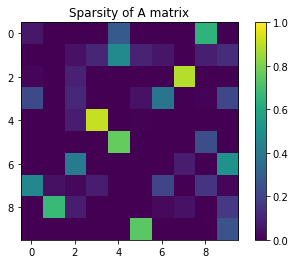
\includegraphics[width=\linewidth]{"report images"/A_sparsity.png}
\end{minipage}
\hfill
\begin{minipage}[H]{0.4\linewidth}
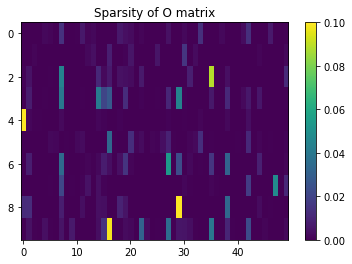
\includegraphics[width=\linewidth]{"report images"/O_sparsity.png}
\end{minipage}%
\end{figure}

From the visualization of the sparsities of these matrices, we see that most of the elements are zero or very close to zero. In the visualization of the sparsity of matrix A, we see that this means that for any given state, there are only a few other states that HMM will transition to. Likewise, for the O matrix, this means that for each states, there are only a few observations that are likely to be emitted. 

\subsection{Visualization of states}

\begin{figure}[H]
\begin{minipage}[H]{0.4\linewidth}
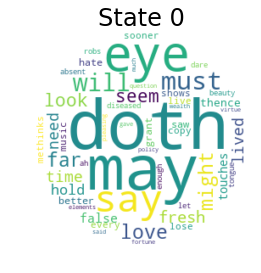
\includegraphics[width=\linewidth]{"report images"/state_0.png}
\end{minipage}
\hfill
\begin{minipage}[H]{0.4\linewidth}
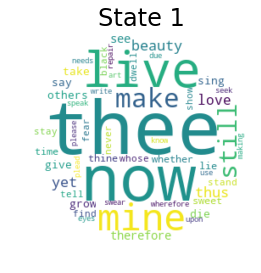
\includegraphics[width=\linewidth]{"report images"/state_1.png}
\end{minipage}%
\end{figure}
\begin{figure}[H]
\begin{minipage}[H]{0.4\linewidth}
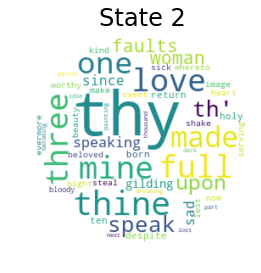
\includegraphics[width=\linewidth]{"report images"/state_2.png}
\end{minipage}
\hfill
\begin{minipage}[H]{0.4\linewidth}
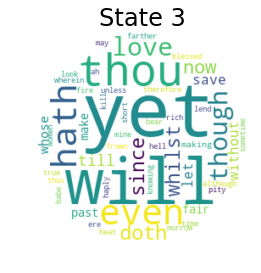
\includegraphics[width=\linewidth]{"report images"/state_3.png}
\end{minipage}%
\end{figure}
\begin{figure}[H]
\begin{minipage}[H]{0.4\linewidth}
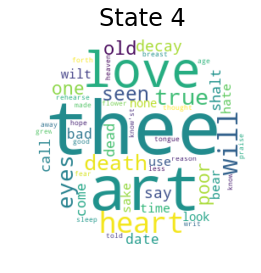
\includegraphics[width=\linewidth]{"report images"/state_4.png}
\end{minipage}
\hfill
\begin{minipage}[H]{0.4\linewidth}
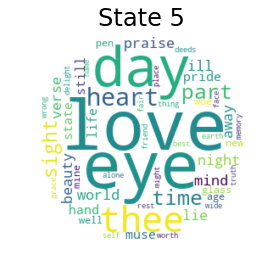
\includegraphics[width=\linewidth]{"report images"/state_5.png}
\end{minipage}%
\end{figure}


 %In addition, for at least 5 hidden states give a list of the top 10 words that associate with this hidden state and state any common features among these groups.
 
 For State 0, we see that the top 10 words associated with this hidden state are eye, doth, may, say, will, must, far, love, seem, and look. Amongst this group, it seems that majority of the words are verbs and other words that might follow a noun.
 
 For State 1, we see that the top 10 words associated with this hidden state are thee, live, now, make, mine, still, love, whether, beauty, and see. This group is mainly made of adjectives or verbs that would generally precede a noun.
 
 For State 2, we see that the top 10 words associated with this hidden state are thy, love, one, mine, thine, full, made, three, speak, and th'. Similar to State 1, this group of words seems to be made of adjectives using to describe a noun or follow a verb.
 
 For State 3, we see that the top 10 words associated with this hidden state are yet, will, hath, thou, since, love, though, even, now, and save. This group of words suggests that this state represents the beginning of prepositional phrase, and words that might follow a noun in the predicate of a sentence.
 
 For State 4, we see that the top 10 words associated with this hidden state are thee, love, art, true, seen, old, decay, heart, death, and will. This group of words represents nouns that are frequently used by Shakespeare and are words that frequently follow verbs or begin a phrase.


\begin{figure}[H]
\centering
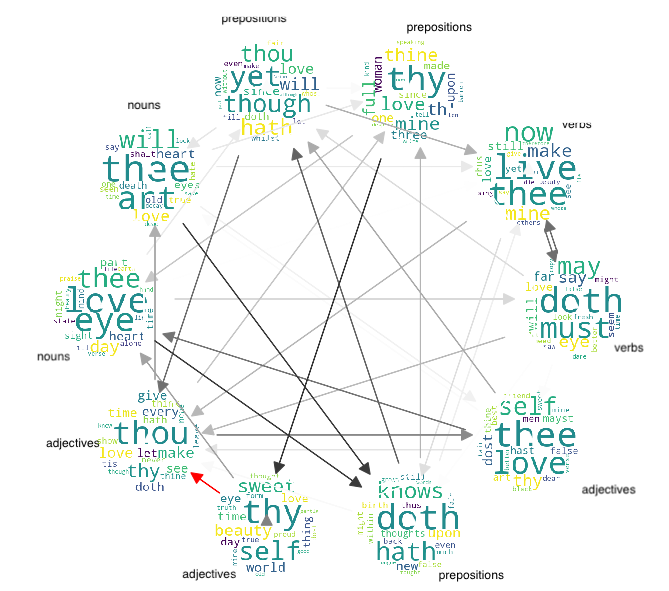
\includegraphics[width=90mm]{"report images"/graph.png}
\caption{Graph of transitions between different states in Hidden Markov Model}
\end{figure}

This graph shows that transitions that we predicted while looking at the individual states are fairly common. We see that the states tend to represent certain parts of speech, and as a result, transition probabilities between certain states reflect the probability of certain parts of speech following one another. For example, we see that the State 4, that we considered the "noun" state often transitions to State 0, which we considered the "verb" state.

From these visualizations, it seems that as HMM learns from the training data, it uses the hidden states to determine different parts of speech, and the transitions are used to determine which parts of speech the model should transition between to mimic the Shakespearean language used in sonnets. With more hidden states, these states would likely extend to include parts of speech with more or less syllables as the machine attempts to account for the iambic pentameter nature of the sonnets. 


\medskip
\medskip
The following sites were used for help with implementation:\\
https://machinelearningmastery.com/text-generation-lstm-recurrent-neural-networks-python-keras/\\
https://machinelearningmastery.com/use-word-embedding-layers-deep-learning-keras/

\end{document}
